\subsection{Scrum of scrums}\label{sub:scrum-of-scrums}
Scrum of Scrums is a framework for scaling scrum across an organization. It allows each scrum team freedom to operate while providing a structure for communicating progress. 

In the ECDAR project the term scrum of scrums was introduced to cooperate transparency between the groups.
In scrum of scrums we do not have daily scrums because the daily scrums is hold in the smaller groups.
The key events in scrum of scrums are the sprint planning sprint review and sprint retrospective.
Look at \autoref{fig:scrum-of-scrums-events} for a more detailed look of the different events between scrum and scrum of scrums.

The multi project is separated in two parts. 
There are five project groups working on the Reveaal part and one group working on the GUI part.
Each group choose a member to attend the scrum of scrums meetings.
The reasoning of this was the number of members attending the meetings would get to big if every group member attended. 
The idea behind this was to keep the meetings as short as possible and because of this each group should hold a meeting internally before sending their committee to the main meeting for the scrum of scrums. 


%Based on that the groups choose a committee to attend the scrum meetings.

\begin{figure}[H]
    \centering
    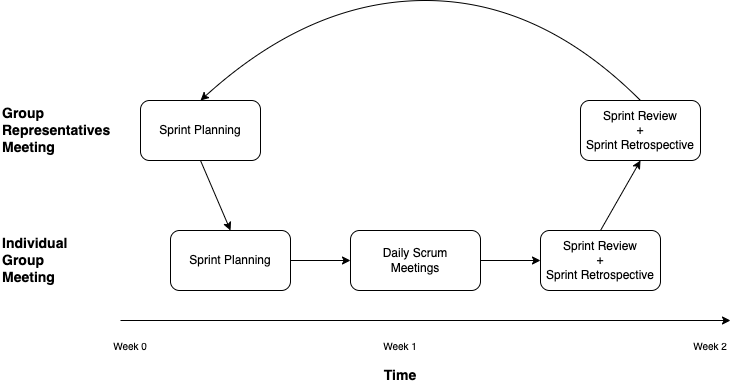
\includegraphics[width=\textwidth]{common/figures/Scrum_of_scrums_schedule.png}
    \caption{The events in a scrum sprint divided between the big scrum of scrums group and the smaller scrum groups}
    \label{fig:scrum-of-scrums-events}
\end{figure}


The multi project is separated in two parts. 
There are five project groups working on the Reveaal part and one group working on the GUI part.
Because of this we have two product owners.
One product owner for the Reveaal part and one for the GUI part.